\documentclass{beamer}

\usepackage[utf8]{inputenc}
\usepackage[spanish]{babel}
\usepackage{lastpage}
\usepackage{subcaption}

\title{Reconstrucción de Huellas Dactilares Digitales Utilizando un Modelo Generativo Adversarial Convolucional}
\author{Cristian Yesid Andrade Hernández}
\institute{Universidad de los Andes}
\date{2020}

\begin{document}

% ==== SLIDE 1 ====
\frame{\titlepage}

\begin{frame}
\frametitle{Introducción}

\begin{figure}[htbp]
\centerline{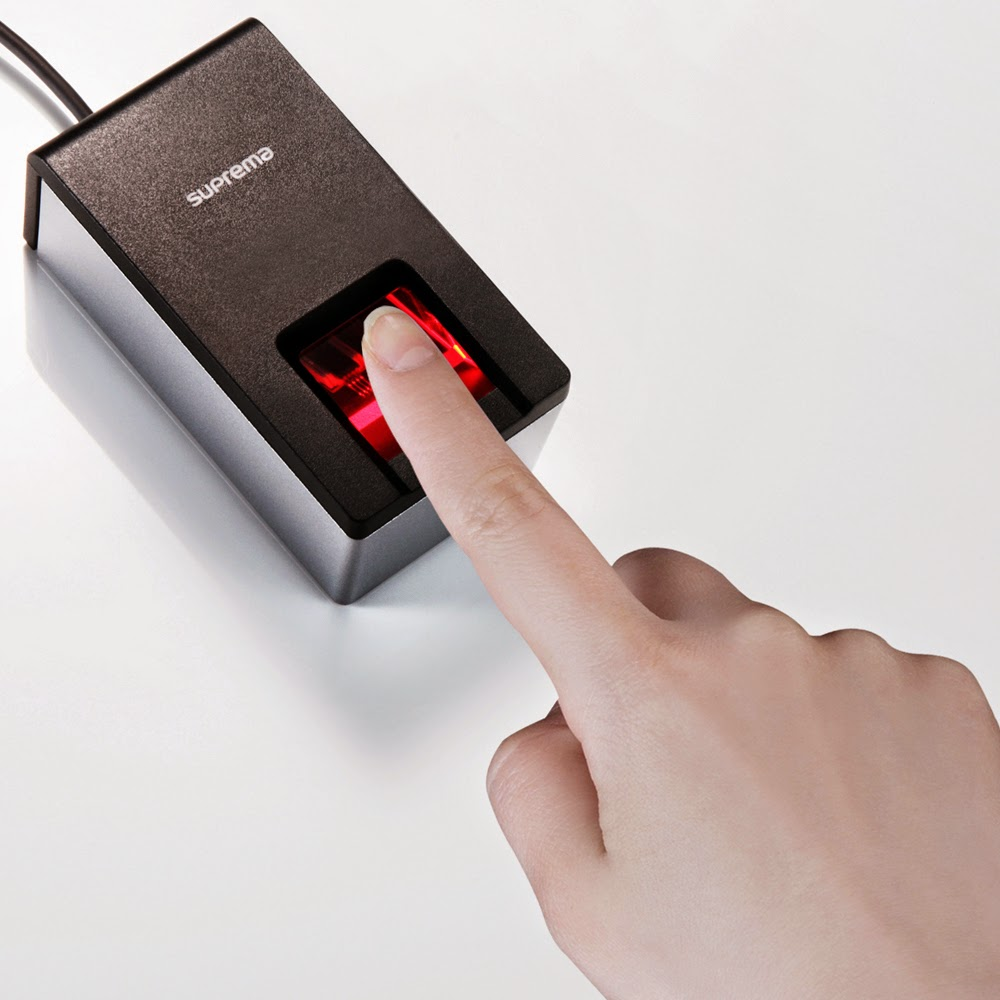
\includegraphics[scale=0.14]{figs/dedo_lector_biometrico.jpg}}
\caption{Lectura Digital de Huella Dactilar}
\label{fig1}
\end{figure}

\end{frame}

% ==== SLIDE 2 ====
\begin{frame}
\frametitle{Introducción}

\begin{figure}[h]
\begin{subfigure}{0.4\textwidth}
  \centering
  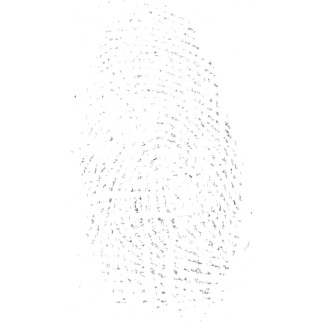
\includegraphics[scale=0.4]{figs/deteriorada_0.png}  
  \caption{Huella Borrosa}
  \label{fig:sub-first}
\end{subfigure}
\begin{subfigure}{0.4\textwidth}
  \centering
  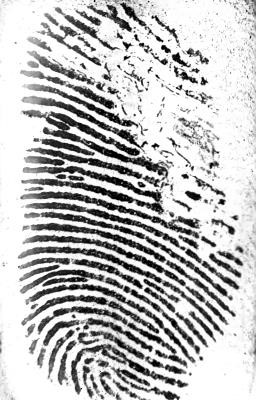
\includegraphics[scale=0.42]{figs/deteriorada_1.jpg}  
  \caption{Huella Incompleta}
  \label{fig:sub-second}
\end{subfigure}

\label{fig:fig}
\end{figure}

\end{frame}

% ==== SLIDE 3 ====
\begin{frame}
\frametitle{Introducción}


\begin{figure}[h]

\begin{subfigure}{0.4\linewidth}
  \centering
  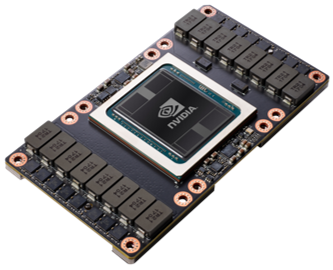
\includegraphics[width=\linewidth]{figs/nvidia_card.png}
  \caption{Capacidad de cómputo}
  \label{fig:sub-first}
\end{subfigure}
\begin{subfigure}{0.8\linewidth}
  \centering
  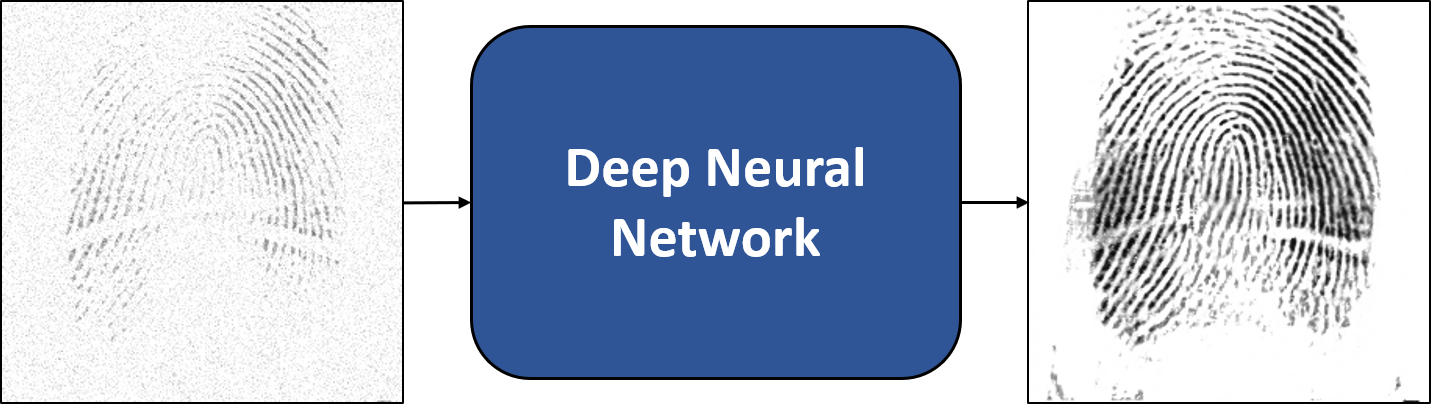
\includegraphics[width=\linewidth]{figs/end_to_end.png}
  \caption{Paradigma End to End}
  \label{fig:sub-second}
\end{subfigure}

\label{fig:fig}
\end{figure}

VIDEO LATEX 9 EN YOUTUBE

\end{frame}

\end{document}